% Chapter 3

\chapter{State-of-the-art Analysis} % Main chapter title
\label{Chapter3} % For referencing the chapter elsewhere, use \ref{Chapter3} 

\lhead{Chapter 3. \emph{State-of-the-art Analysis}} % This is for the header on each page - perhaps a shortened title

%----------------------------------------------------------------------------------------
In this section, we discuss the core requirements and other factors that are required to be solved to provide a viable solution. There are plenty of alternatives available under each topic. Thus, we consider solutions that are mostly relevant, widely available and used in the related domain, industry as well as findings from latest related research works. This analysis enables us to choose the best data treatment technique and programming model that are well suited and to select the core design aspects that need to be considered. To make selections with adequate foundation, we first discuss the requirements and then compare each alternatives with respect to the requirements. 
\section{Fundamentals }
\label{sec:fundamentals}
Essential requirements that need to be met by the system are defined in Section \ref{sec:motivation} and additional aspects that needs to be solved by new scalable ETL tools are mentioned in Section \ref{sec:requirements}. To summarize, the system should be execute data preparation on large data (R1), scalable i.e. able to distribute the work according to the load  (R2), real-time responsive in interactive context (R3), efficient on iterative execution (R4). Further, Separation between logical and physical implementation of data cleaning operations becomes an optimization requirement (R5), providing flexibility (R6) behaves as a functional improvement requirement and solution as a service (R7) to provide a general integral solution.  The following important topics need to be carefully analyzed with respect to problem space to create a fit-for-purpose solution. 

\subsection{Data ingestion technique}
Data ingestion technique is a data processing model or the routine how the input data is initially received and represented to be processed. The most frequently used data ingestion or treatment techniques in big data paradigm are batch processing, stream processing and micro-batch processing \cite{dataflow}. Batch processing is a technique of treating the input data as a collection of data where the input data is assumed as fully available to be processed \cite{Sims-387}. Batch processing is generally used as store-first, process-second model of large and of identical types. In contrast, stream processing is a data processing model where data is treated as streams of data \cite{beyondbatchprocessing}. For example, a data stream can be generated based on event-by-event or complex-event-streams. They are not considered to be pre-available before it is processed and they can be out-of-order, out-of-streams \cite{beyondbatchprocessing} \cite{Sims-387}. Stream processing is mainly aimed to do continuous processing on similar data streams in real-time \cite{8reqofrealtime}. Micro-batching is a combined version of batch processing and stream processing, which is to treat data as sequence of small batches of streams. Streams can be delayed to collect small batches or batch inputs can be split into small set of streams to become micro-batches. 
\begin{center}
	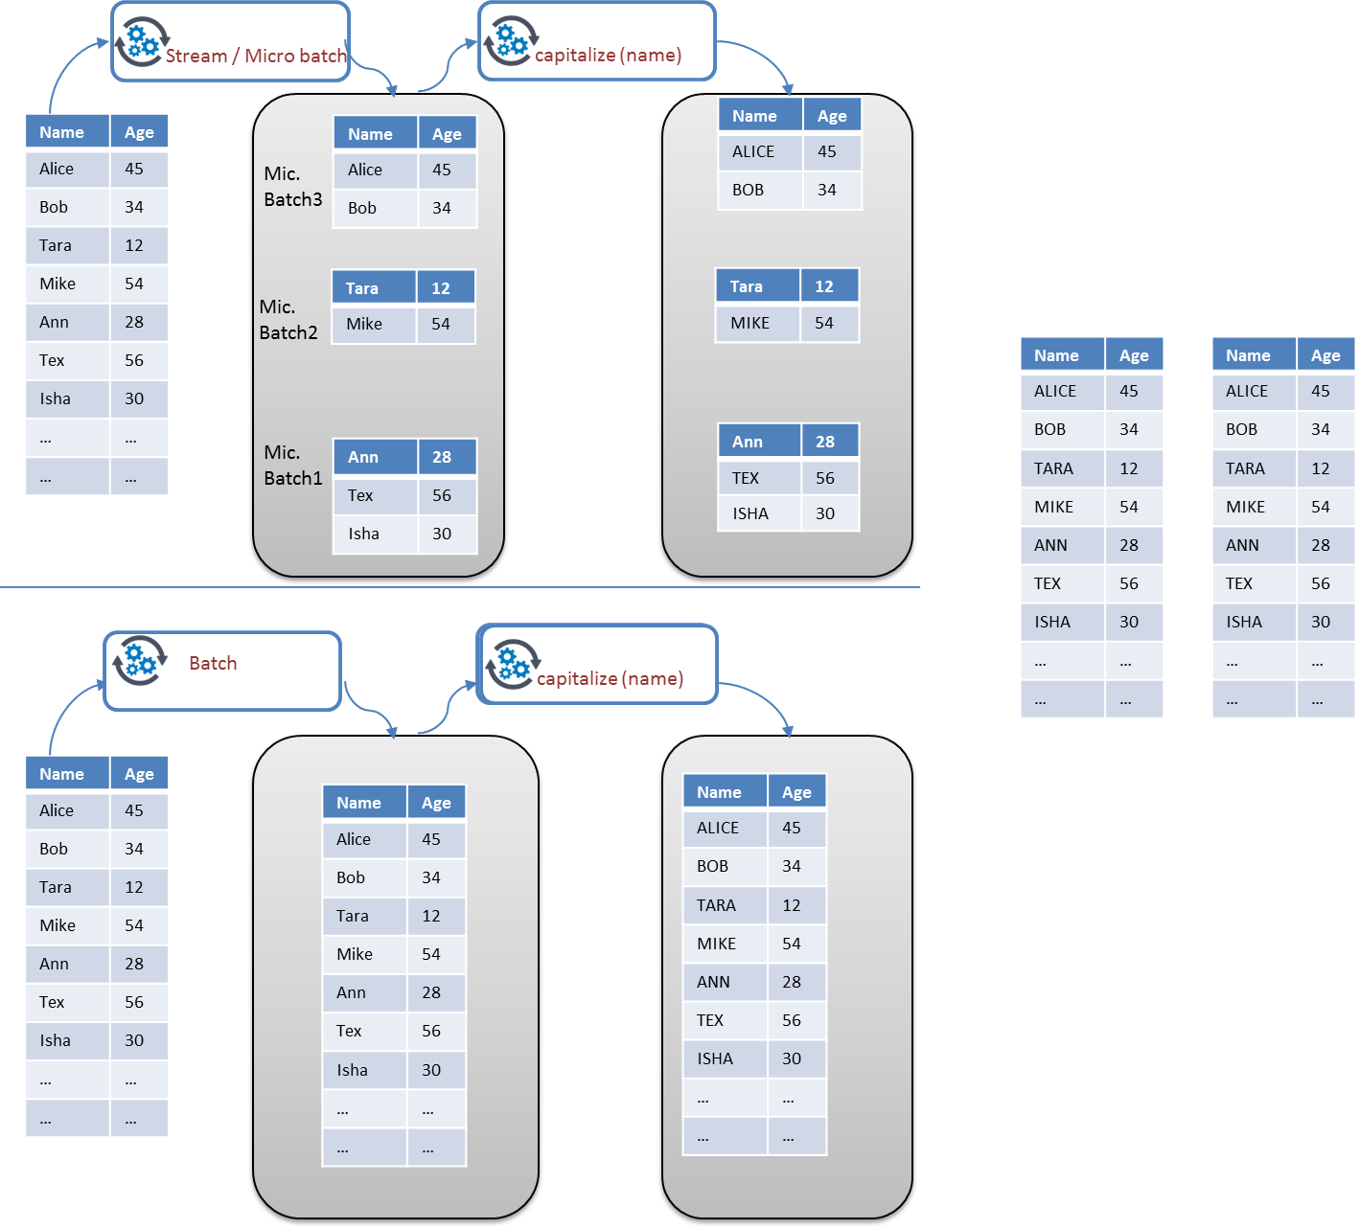
\includegraphics[width=38em]{./Figures/batch-cleaning-right}
	\begin{figure}[htbp]
    \caption{Data cleaning in different data treatment techniques performed as expected}
    \label{fig:streamcorrect}
	\end{figure}
\end{center}
 On small intervals, the incoming stream is collected to a chunk of data and delivered to be processed as a small batch of input \cite{beyondbatchprocessing}. 
 
 Choice of appropriate data ingestion technique is essential to receive precise output. Given that, on today's date, the messy data we target to process in open data context are usually text-files or spreadsheets. These data are already available and need to be processed to create RDF data. 
 Since we need to process large files, the right choice of data ingestion is important. Streaming or Micro batching data can be a solution to overcome the problem of processing large files. However, since we need to perform ETL operations on table like data, it will not result in expected output in all instances. Figure \ref{fig:streamcorrect} shows that streaming or micro batching can provide expected solution when simple data cleaning operations performed independent from other row values such as capitalize, lower case and upper case etc. 
 \begin{center}
	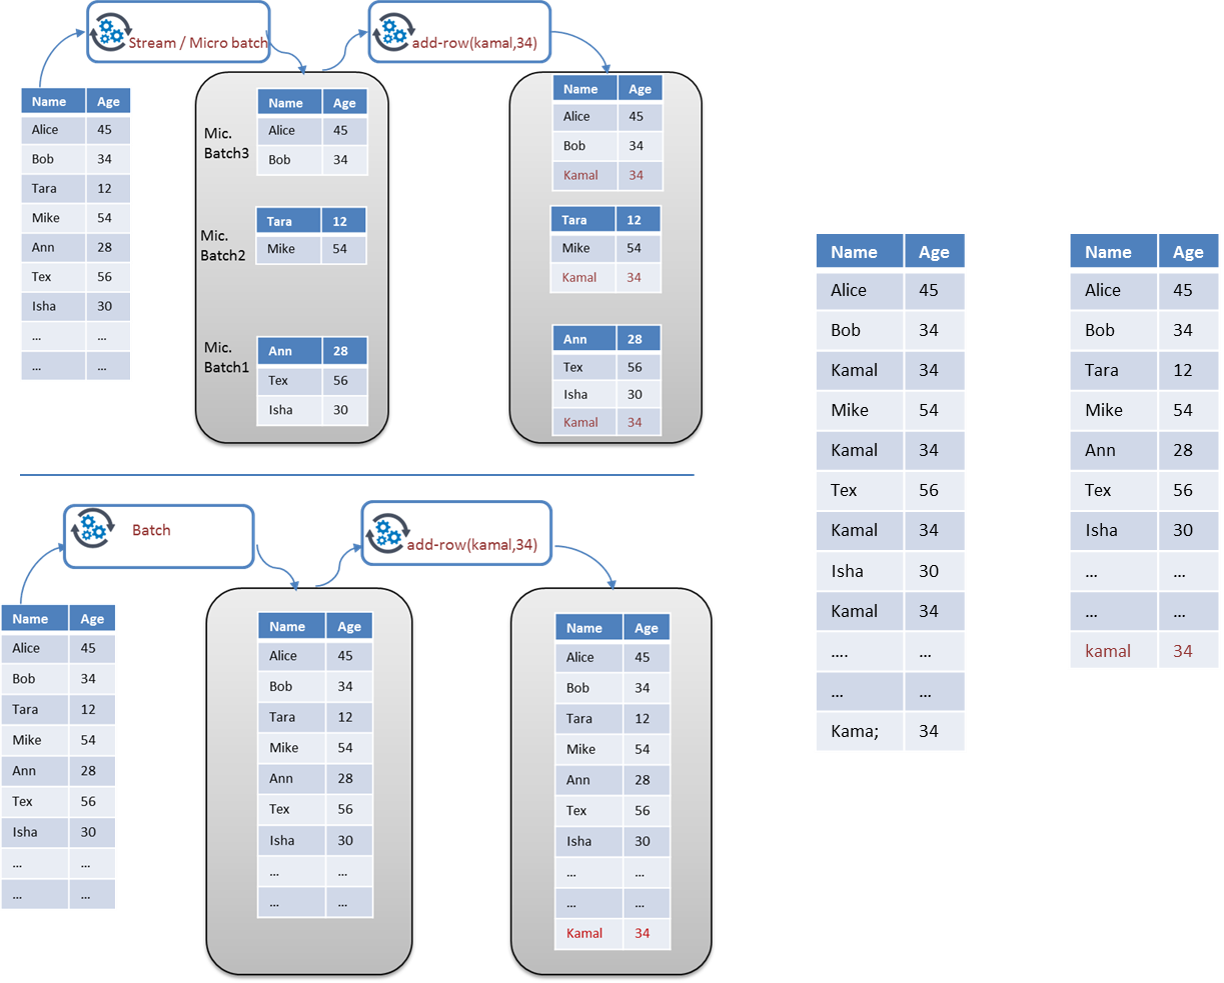
\includegraphics[width=38em]{./Figures/batch-cleaning-wrong}
	\begin{figure}[htbp]
    \caption{Data cleaning on a faulty data treatment results in unexpected result}
    \label{fig:stream-wrong}
	\end{figure}
\end{center}
 However, it will result in wrong output when collective operations or row dependent operations like add-row is performed on data as shown in Figure \ref{fig:stream-wrong}. Figure \ref{fig:stream-wrong} illustrates an add-row operation performed on a simple tabular data. When the data is ingested as streams, which are independent from each other, the transformation pipelines are performed on all streams which result in redundant addition of rows, whereas in batch ingestion the data is treated as a single batch and operation is performed safely. Performing complex schema-based data cleaning will be cumbersome and error-prone in stream or micro batch processing. Seeing that, we conclude that ingesting those messy files as batch is the most suitable and precise method for data cleaning. This adds efficient batch-processing (R5) to our requirements. This implicitly requires our solution to process large file as a batch input and respond in real-time. In contrast, batch processing is typically performed as batch jobs which are independent from user \cite{beyondbatchprocessing} and take longer duration (from few minutes to hour) to complete. Despite, we attempt to solve this in near-real-time (i.e within few seconds to few minutes) which can still afford to have active user interaction and perform batch processing. 
 \subsection{Programming Model}
Another important foundation to analyze is the programming model of our solution. As a whole the solution should be able to perform iterative cleaning operations, that can work as batch processing solution and respond in near-real-time. Distributed data paralleling is the most widely used computation model in big data that provides load balancing, fault tolerance of input data \cite{Jackson2015517} and scalability. To decide the most suitable programming model that can work with distributed data parallelizing according to our requirements, we analyzed alternatives that are widely used in research, industry and actively maintained. Specifically, we focused on studies and system that can provide simple distributed computing means which should be a near-real-time responsive system to respond to interacting user, as well an efficient and effective to perform iterative jobs. 
\subsubsection{MapReduce and Apache Hadoop}
MapReduce is the pioneer of distributed data processing techniques. It is a programming model proposed by Google. By providing two primary parallel methods over distributed data (map and reduce) it achieves load balancing fault tolerance. Apache Hadoop\footnote{http://hadoop.apache.org/} is an open source implementation of MapReduce, which was a game changer in big data domain. Apache Hadoop also provided important distributed programming components such as  Hasoop Distributed File System (HDFS) and YARN Resource Manager. However, MapReduce was later identified for its draw-backs on having huge File Input/Output (I/O) to store and load intermediate data. It is extremely slow and resource consuming when iterative operations are executed as pipeline of operations. Figure \ref{fig:hadoop-high-io} shows how iterative jobs result in high I/O in MapReduce, since every stage is going through dish write and read. Further, Reduce operation can be only started only after all map jobs are completed.
 \begin{center}
	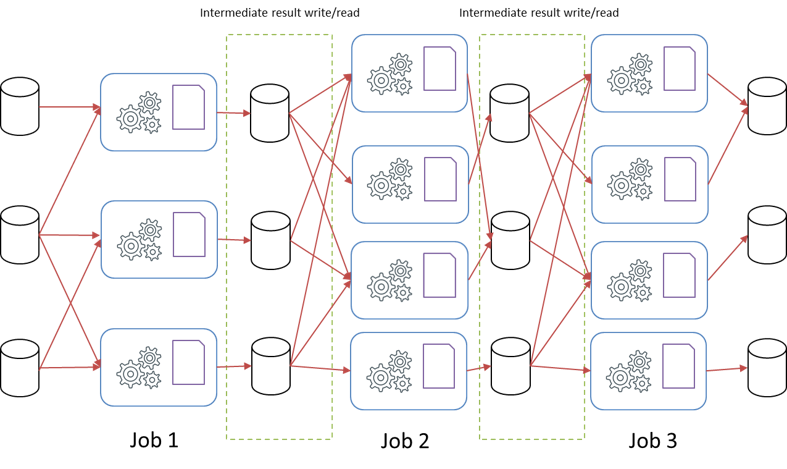
\includegraphics[width=32em]{./Figures/hadoop-high-io}
	\begin{figure}[htbp]
    \caption{High Input/Output behavior when iterative jobs performed on MapReduce}
    \label{fig:hadoop-high-io}
	\end{figure}
\end{center}
 This leads to a long execution time. Hence, it doesn't suit our requirements of supporting iterative operations as a pipeline and not a near-real-time responsive programming model. 
\subsubsection{Dryad and DryadLINQ}
Dryad\footnote{http://research.microsoft.com/en-us/projects/dryad/} is a general purpose framework for distributed, parallel-data applications created at Microsoft Research. Dryad, mainly focused on providing simplified programming model for parallel and distributed application development and their scalability, reliability and efficiency \cite{DRYAD}. A Dryad application consists \textit{vertices} that communicate to \textit{channels}, which eventually creates dataflow graph. Dryad supports executing multiple operations as a Directed Acyclic Graph (DAG) that eliminated the problems addressed by MapReduce. Further, Dryal also provided not only Map, Reduce, but also more features like sort, group. DryadLINQ\footnote{http://research.microsoft.com/en-us/projects/DryadLINQ/} is a powerful general purpose programming model provided by Dryad. DryadLINQ provides a simple declarative programming interface by supporting general-purpose imparative and declarative operations on data-sets within a traditional high-level programming language \cite{DryadLINQ} by utilizing Language-Integrated Query (LINQ) expressions. This enables flexible and efficient distributed in programming languages such as C\#, VB and F\#. Although, it is not available as an open source or commercialized solution, rather internally used in Microsoft. Dryad also inherits the performance penalty from MapReduce, as data must be reloaded from disk \cite{Spark}.
\subsubsection{Apache Spark and Resilient Distributed Dataset}
\label{sec:spark}

\textbf{In-memory cluster computing} 

Apache Spark\footnote{http://spark.apache.org/} is today's "de-facto" of big data, a general purpose distributed data processing framework, which is built to meet recent big data requirements such as iterative jobs and interactive analysis \cite{Spark}.  Spark sets a new computing paradigm called \textit{in-memory cluster computing} \cite{RDD} , using its main abstraction called \textit{resilient distributed dataset}, which holds a read-only representation of data object distributed across a set of machines (i.e. on Distributed Shared Memory (DSM)), that is fault tolerant \cite{RDD}. This eliminates the drawback of  having high I/O by not storing and loading back intermediate results of every iteration as depicted in Figure \ref{fig:in-memory-computing}.
 \begin{center}
	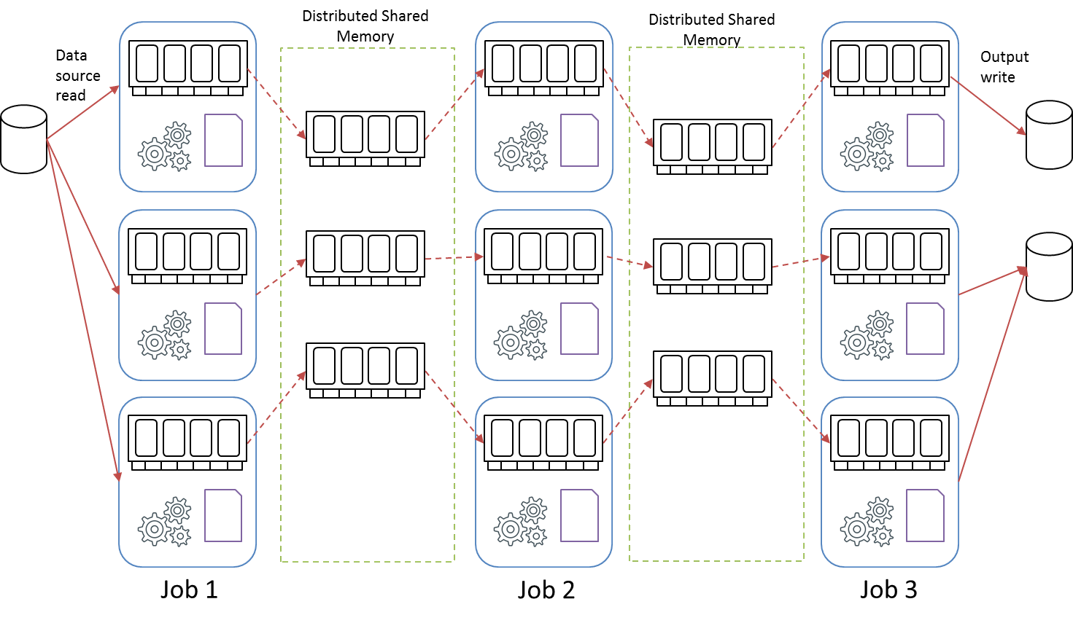
\includegraphics[width=32em]{./Figures/in-memory-computing}
	\begin{figure}[htbp]
    \caption{Behavior of in-memory-computing with iterative jobs}
    \label{fig:in-memory-computing}
	\end{figure}
\end{center}
Spark's another main aspect is parallel operations provided by spark, that can execute in parallel on different data partitions. Spark is claimed to be 10x - 100x faster than Hadoop in iterative applications \cite{Spark}\cite{RDD} \citep{clashoftitians}, by benefiting from Spark's programming model. Spark also provides distributed cache and shared variables to reuse computed resources that suits iterative computation. Spark also utilizes Hadoop's HDFS and YARN implementations. Spark is also considered as the open sourced implementation of research work done in Dryad. Spark also provides simplified language integration and functional programming syntax to write distributed computing applications \cite{Spark}\cite{Spark-improvements} and executes Spark jobs in DAG similar to DryadLINQ. 

The primary difference between Dryad and Spark is that Dryad cannot efficiently perform problems of iterative algorithms \cite{spark-vs-stratosphere}. In contrast to DryadLINQ, Spark lets RDDs to be persisted in memory across parallel operations. Further, Spark provides additional features like shared variables and cache which were not supported by Dryad \cite{Spark}.

\textbf{Spark's Strong Eco System}

Spark is one of the most widely used open source big data processing engine \cite{Spark-scalable}. Spark provides fully featured functional Application Programming Interface (API) in multiple languages Scala, Python, Java and R. In addition, Spark also evolved with providing underlying support for distributed processing of tabular data using Spark SQL \cite{SparkSQL}, graph data using GraphX \cite{GraphX}. Further, Spark also provides large scale machine learning libraries and support for stream and micro-batch processing. Figure \ref{fig:spark-prog-models} shows the main programming components provided by Spark eco system. 
 \begin{center}
	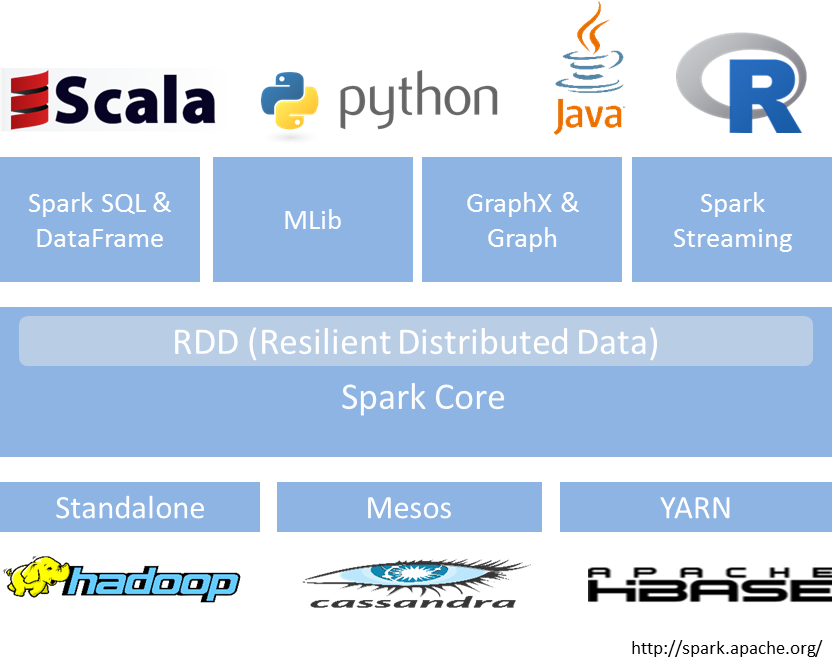
\includegraphics[width=32em]{./Figures/spark-programming-components}
	\begin{figure}[htbp]
    \caption{Programming components of Apache Spark Eco System}
    \label{fig:spark-prog-models}
	\end{figure}
\end{center}

\textbf{Lazy-evaluation of Spark Jobs} 

Moreover, RDD is an immutable distributed collection of objects. Making use of immutable object user can easily perform side-effect-free computation. Spark provides two types of operations that can be executed on RDD namely \textit{transformations} and \textit{actions}. \textit{Transformations} create a new RDD from previous one, whereas \textit{Actions} compute results based on a RDD and return it to driver program or store in external storage system (e.g. HDFS). Execution of a Spark job with multiple tasks are performed \textit{lazily}, such that the transformations are actually executed only when it reach an action. Until a pipeline reaches an action, the transformations are stored only as a meta-data \cite{learnspark}. When an action is reached Spark sees the whole chain of transformations, and compute the result needed. This provides a great level of optimization of jobs with pipeline of tasks, specially when large data is processed. 

\textbf{Scalable runtime architecture of Spark}

Spark uses master/slave architecture during distributed mode. It uses one central coordinator and many distributed workers to execute a given job. The central coordinator or master process is called \textit{Driver}. A driver communicates to large number of distributed workers which are called \textit{executors}. They compose a \textit{Spark application} which is launched on cluster of machines using an external service called \textit{cluster manager}. Spark works with cluster managers such Hadoop YARN, Apache Mesos and has its own standalone manager. 
\begin{center}
	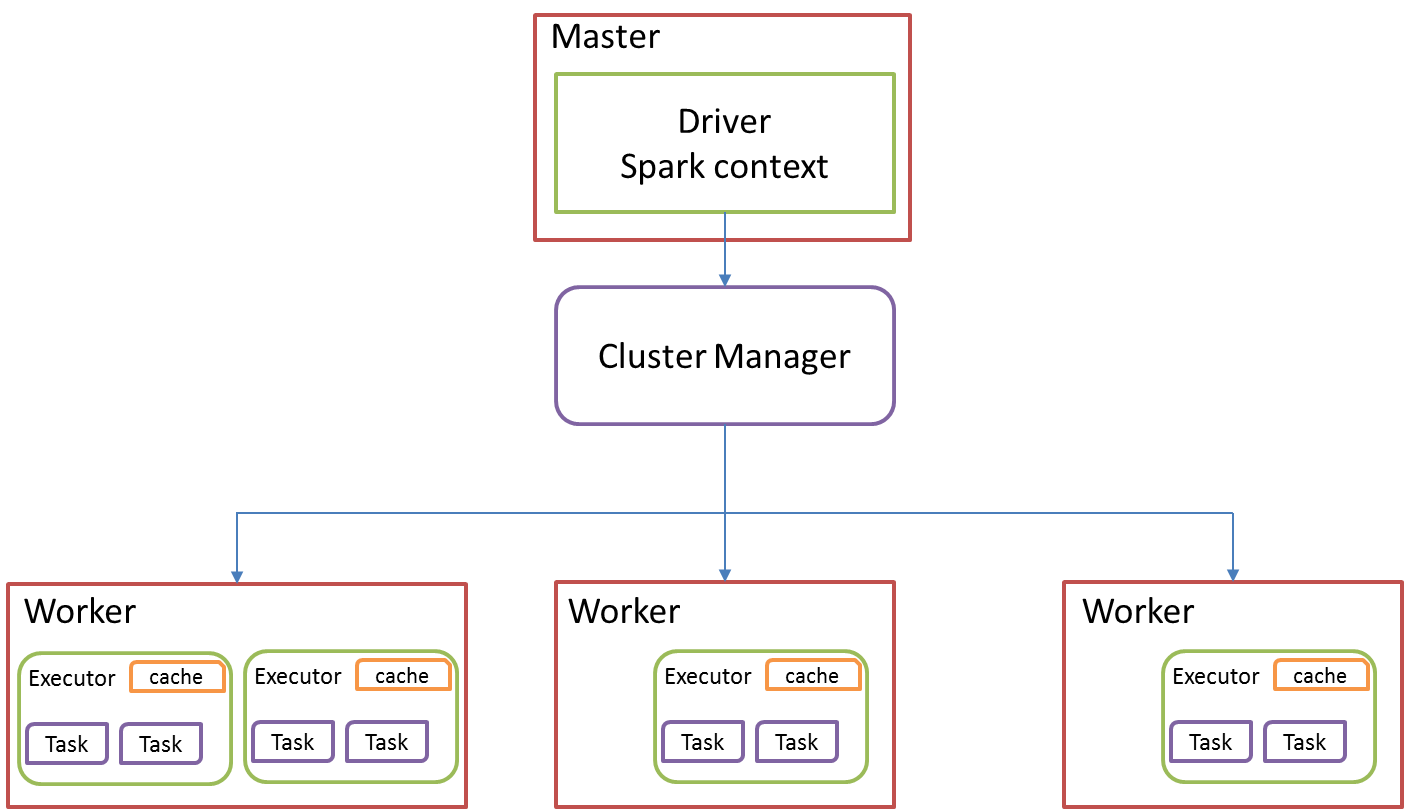
\includegraphics[width=28em]{./Figures/spark-master-slave}
	\begin{figure}[htbp]
    \caption{Spark's runtime architecture in distributed mode}
    \label{fig:spark-masterslave}
	\end{figure}
\end{center}
\textit{Driver} is the process which creates a SparkContext, creates RDD, converts user programs into spark\'s physical execution tasks, and creates logical representation of them in a DAG form and inform them to distributed workers. \textit{Executors} are the worker processes that performs individual tasks in a job. Executors are launched when a spark application is started and they typically run till the spark application stops unless there is a failure. Executors register themselves with driver process and receive and respond to driver according to the tasks given. Driver handles the rest.  Spark provides scripts to submit spark applications to cluster which is called \textit{spark-submit}. According to the configuration in spark-submit a spark cluster is launched. This lets the application to scale according to the cluster configurations mentioned in spark-submit. 

From these analysis, we can safely conclude that Apache Spark fits our purpose well better than other systems. Hence, we choose Apache Spark as our base platform and in-memory computing on RDD as our programming model to perform scalable, interactive and iterative open data cleaning.
\section{Summary}
After analyzing important requirements and solution fundamentals, we have noted that batch-processing is the correct ingesting method to do data cleaning on offline messy data. Secondly, in-memory computing and distributed data parallelizatoin from Apache Spark can be exploited to perform interactive, iterative data cleaning. 